%!TEX root = ../Thesis.tex

\section{Introduction}
\label{sec:introduction2}%

The past fifty years have been marked by the evolution of computers and an enormous availability of computational power. This has boosted the development of computational methods and their application in engineering. The most popular computational method is the finite element method (FEM), however around 1970 the engineering community started to develop the boundary element method (BEM).

The term \emph{Boundary Element Method} was coined in 1977 in three publications: Banerjee and Butterfield, Brebbia and Dominguez, and Dominguez. The mathematical foundations were established by Betti in 1872 and Somigliana in 1886 for elasticity problems, while Green in 1828 and Fredholm in 1903 made foundational contributions to potential problems.

A fair question to ask is "why do we need the BEM since we already have the FEM that solves engineering problems?". The answer is that modeling with finite elements can be ineffective and laborious for certain classes of problems. So the FEM, despite the generality of its application in engineering problems, is not free of drawbacks. The most important advantages of preferring BEM over FEM are:
\begin{enumerate}
  \item The solution is mathematically expressed as a continuous mathematical formula, namely a Boundary Integral Equation (BIE). Therefore the associated numerical method, the BEM, benefits of a discretization only over the boundary $\Gamma$ of the problem domain $\Omega$, leading to a significant reduction in the number of degrees of freedom of the numerical model (see Fig~\ref{fig:bem-fem-mesh}).
  \begin{figure}[H]
    \centering
    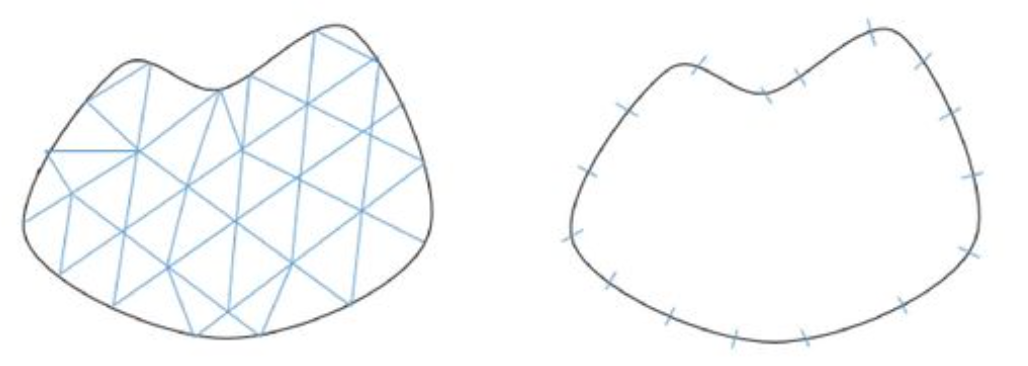
\includegraphics[width=0.8\textwidth]{bem-fem-mesh.png}
    \caption{FEM versus BEM domain discretization.}
    \label{fig:bem-fem-mesh}
  \end{figure}
  \item The method is particularly effective in computing accurately the derivatives of the field function (e.g., fluxes, strain, stresses, moments).  Instead, in FE methods the accuracy drops considerably in areas of large gradients.

  However, we mention that in mixed Neumann Dirichlet problems with Lipschitz domain there arises an issue when considering continuous elements. A possible solution is the so-called double node technique, where, thanks to the splitting of a physical node into more computational nodes, continuity is preserved only on the solution, while its normal gradient is allowed to have a jump across physical edges.
  
  \item For infinite domains, the problem is formulated simply as an exterior one. In this manner computer programs developed for finite domains can be used, with just a few modifications, to solve problems in infinite domains. This is not possible with the FEM.
  \item The method is well suited for solving problems in domains with geometric peculiarities, such as cracks. Moreover, BEM is more feasible for problems described by differential equations of fourth or higher order (e.g., plate equation).
\end{enumerate}

On the other hand, the BEM exhibits the following inherent main disadvantages:
\begin{enumerate}
\setcounter{enumi}{5}
  \item Application of the BEM requires the establishment of the BIE. This is possible only if the problem is linear and its fundamental solution can be established, such as for Laplace equation, Helmholtz equation, and Stokes system. Hence, the method cannot be used for problems whose fundamental solution is either unknown or cannot be determined. Such are, for example, problems described by differential equations with variable coefficients.
  \item The numerical implementation of the BEM results in systems of linear algebraic equations whose coefficient matrices are fully populated and nonsymmetrical. Moreover, if one considers mixed Neumann Dirichlet boundary value problems the final linear system is generally ill conditioned. In a FEM model, however, the corresponding matrices have some very nice properties, they are banded and symmetric. This drawback of the BEM is counterbalanced by a smaller dimension of its matrices (see Figure~\ref{fig:bem-fem-grid}).
  \begin{figure}[H]
    \centering
    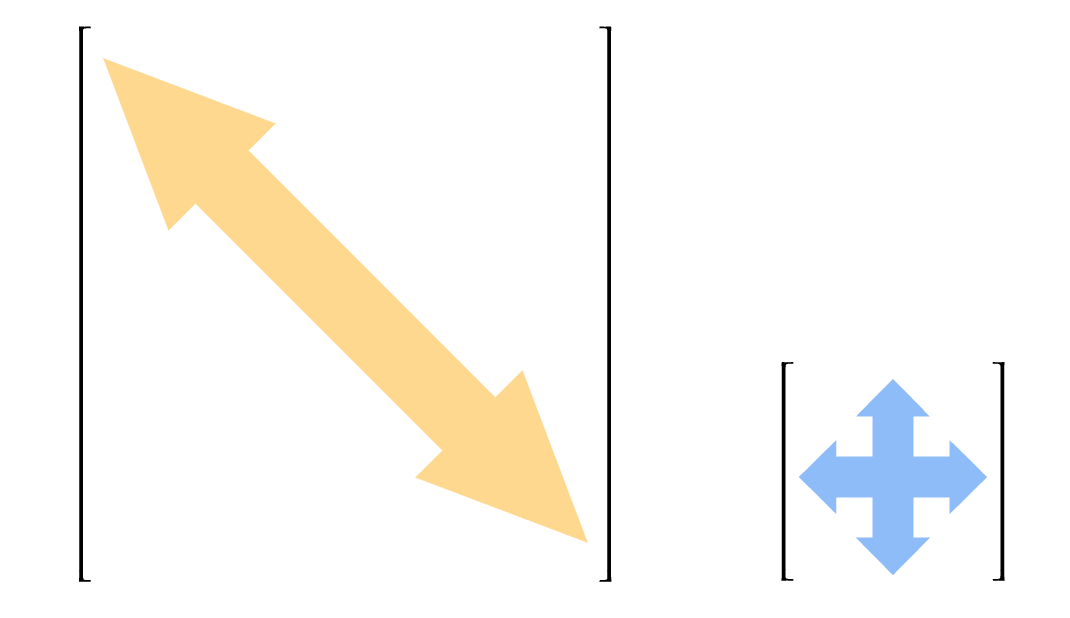
\includegraphics[width=0.6\textwidth]{bem-fem-grid.png}
    \caption{FEM versus BEM coefficient matrix.}
    \label{fig:bem-fem-grid}
  \end{figure}
\end{enumerate}

Nowadays, boundary integral formulation have been applied to problems involving hydrodynamic flows (e.g., Figure~\ref{fig:fish}), flow around aerodynamic lifting bodies, structural mechanics, electrostatics, quantum mechanics, and acoustics (e.g., Figure~\ref{fig:dummy-head}). See~\cite{Attilio} for more delailed explanations. 

\begin{figure}[H]
    \centering
    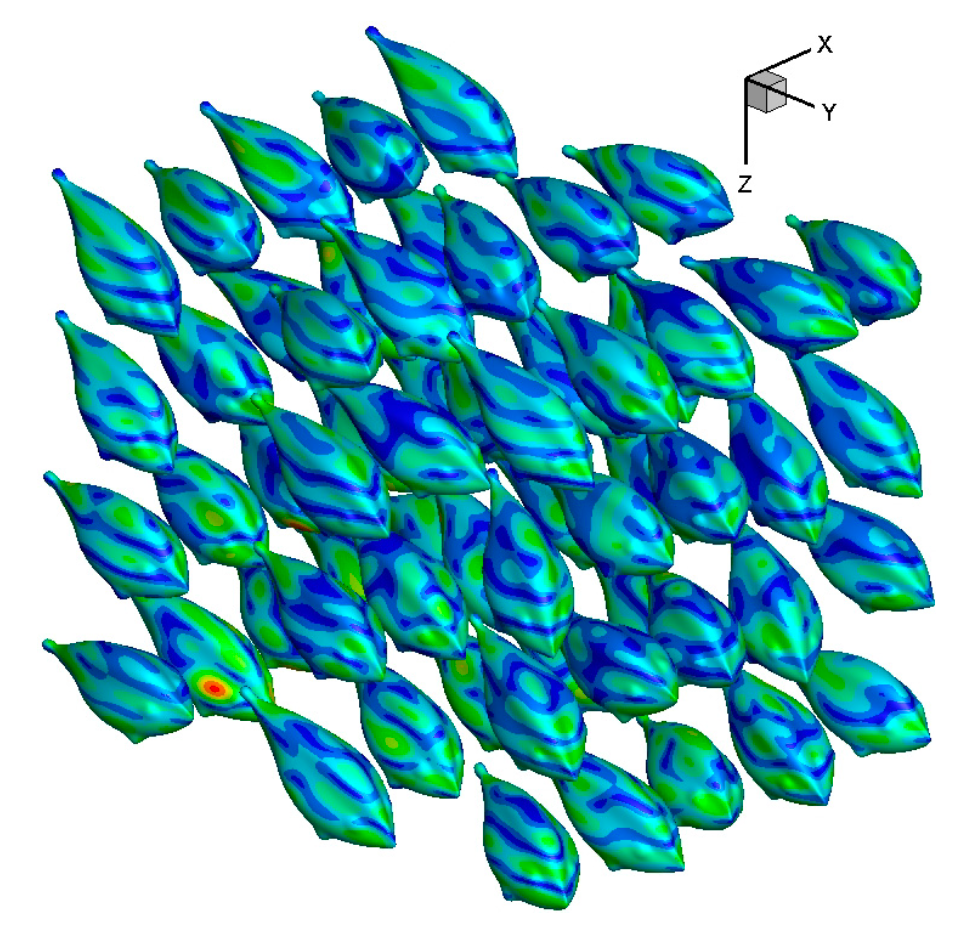
\includegraphics[width=0.3\textwidth]{fish}
    \caption{Scattering of a multiple fish model.} 
    \label{fig:fish}
\end{figure}

\begin{figure}[H]
    \centering
    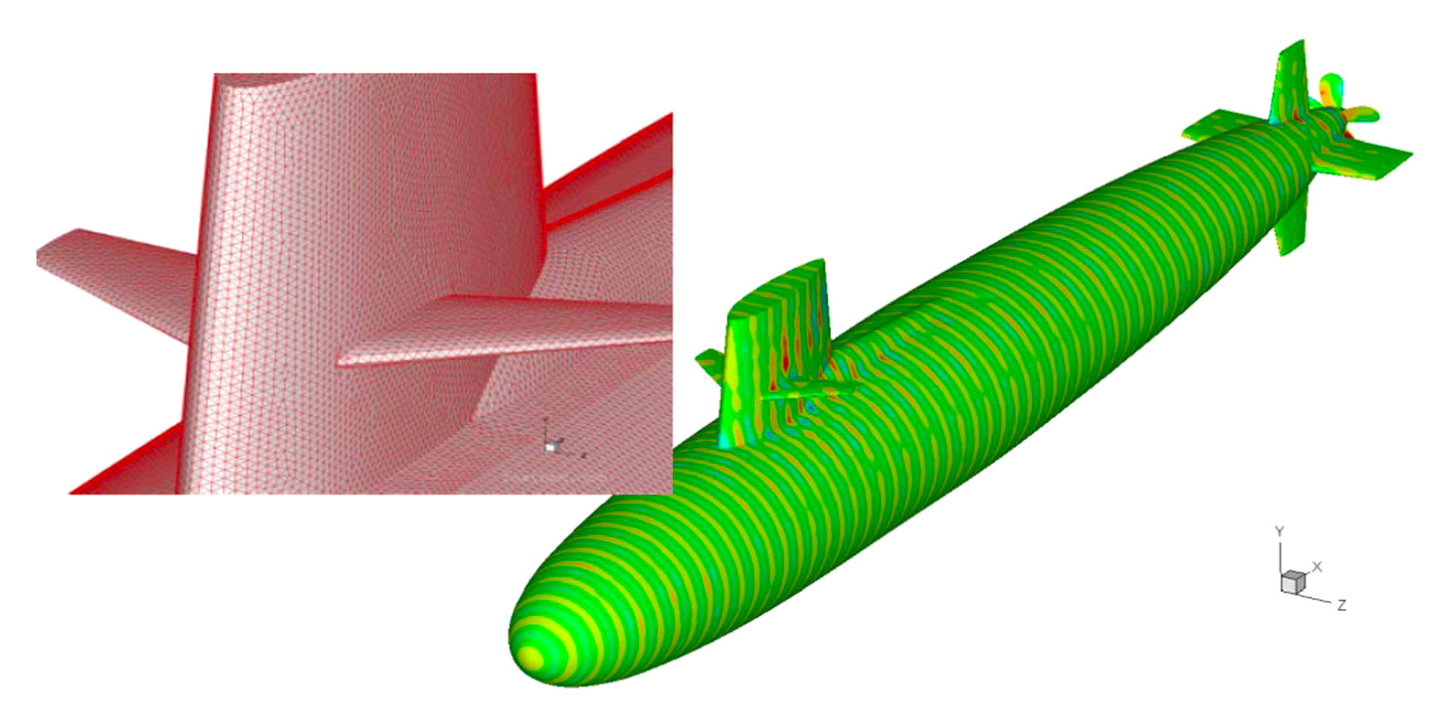
\includegraphics[width=0.5\textwidth]{skipjack} 
    \qquad \qquad
    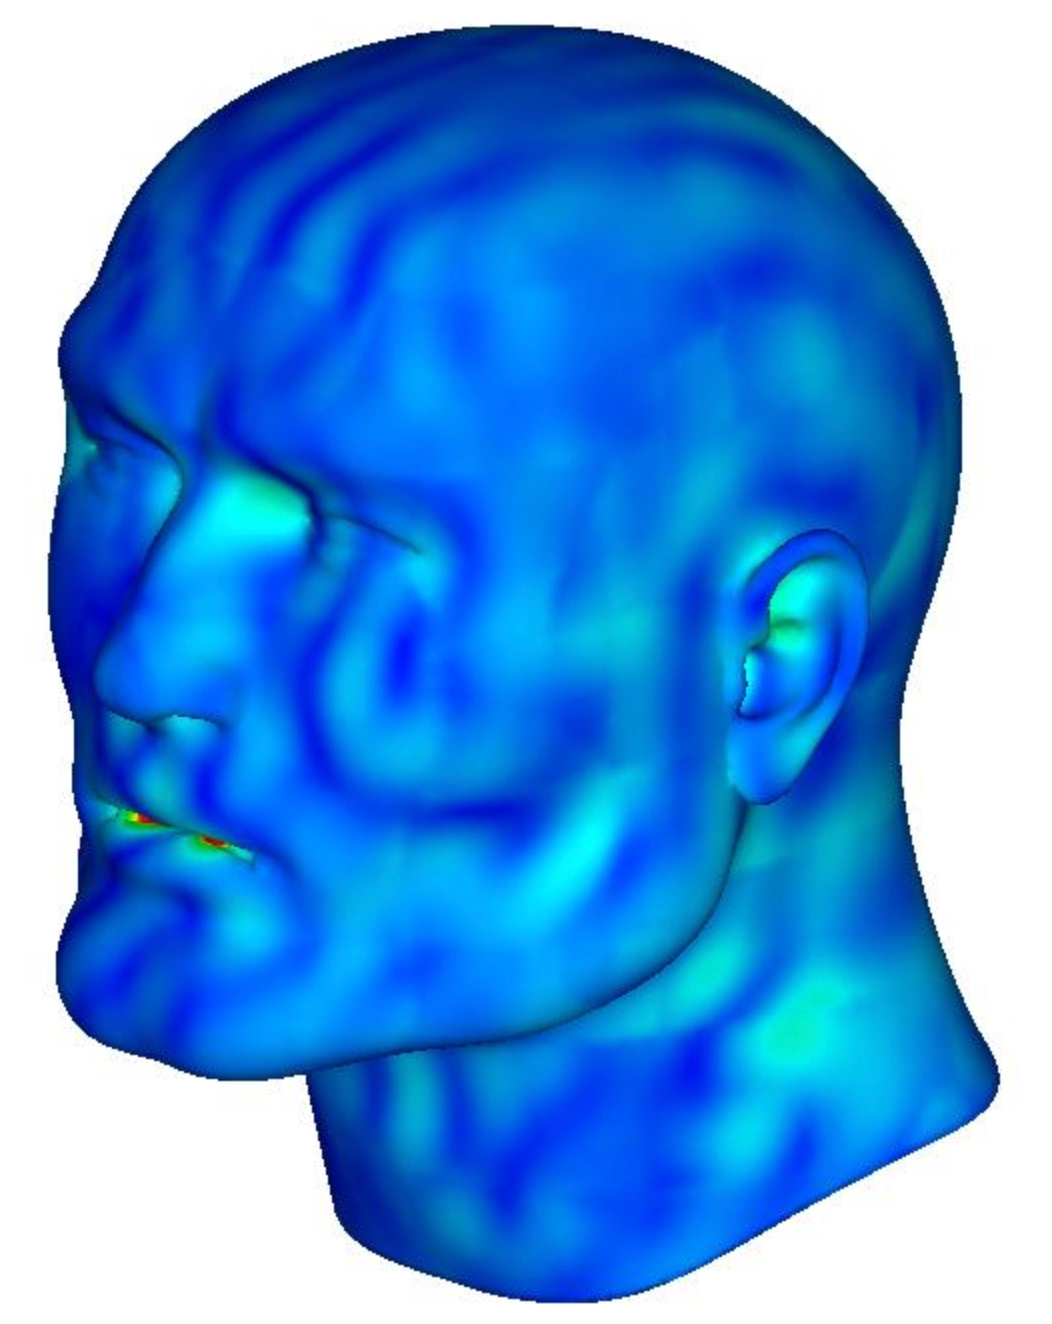
\includegraphics[width=0.2\textwidth]{dummy-head}
    \caption{(Left) BEM model of the Skipjack submarine impinged upon by an incident wave in the direction $(1, 0, \text{-}1)$. (Right) BEM mesh and sound-pressure plots for a human-head model.} 
    \label{fig:dummy-head}
\end{figure}

In this chapter we are going to present the theoretical background and several numerical application of the BEM, mainly referring to~\cite{sbemKatsi}.

\newpage

\section{Boundary Integral Equations}
\label{sec:boundary_integral_equations}%

We consider a bounded open domain $\Omega\subseteq\RR^2$ with Lipschitz boundary $\Gamma=\partial\Omega$, and we want to solve engineering problems described by the potential equation
\begin{equation}
\label{eq:poisson-eq}
\Delta u=f(x,y)\qquad \text{in }\Omega.
\end{equation}

This is the Poisson equation, which for $f=0$ is known as the Laplace equation. Here $u:\RR^2\to\RR$ is the potential produced at a point $(x,y)$ in the domain $\Omega$ due to a source $f(x,y)$. Usually, Eq.~\eqref{eq:poisson-eq} is coupled with the following boundary conditions:
\begin{align}
&
\text{Dirichlet b.c.} 
&& 
{\renewcommand*{\arraystretch}{1}
\begin{array}{l}
u=\overline{u}
\end{array}} 
&&
{\renewcommand*{\arraystretch}{1}
\begin{array}{l}
\text{on }\Gamma
\end{array}} 
\label{eq:Dbc} 
\\
& && && \nonumber\\
&
\text{Neumann b.c.} 
&& 
{\renewcommand*{\arraystretch}{1}
\begin{array}{l}
\displaystyle\frac{\partial u}{\partial n}=\overline{u}_n
\end{array}}
&&
{\renewcommand*{\arraystretch}{1}
\begin{array}{l}
\text{on }\Gamma
\end{array}} 
\label{eq:Nbc} 
\\
& && && \nonumber\\
&
\text{Mixed b.c.} 
&&
{\renewcommand*{\arraystretch}{1.5}
\begin{array}{l}
u=\overline{u} \\
\displaystyle\frac{\partial u}{\partial n}=\overline{u}_n
\end{array}}
&&
{\renewcommand*{\arraystretch}{1.5}
\begin{array}{l}
\text{on }\Gamma_1 \\
\text{on }\Gamma_2
\end{array}}
\label{eq:Mbc}
\end{align}

where $\displaystyle \frac{\partial u}{\partial n}=\nabla u\cdot \nv $, $\Gamma_1\cup\Gamma_2=\Gamma$ and $\Gamma_1\cap\Gamma_2=\varnothing$.

\subsection{Fundamental Solution}
\label{sub:fundamental_solution}%

Before dealing with a bounded domain, let us solve the Poisson equation in the whole $\RR^2$. As phisics suggests, we first compute the potential at point $\xv\in\RR^2$ generated by a unit point source placed at point $\yv$. In other words, the load $f(\xv)$ is the \emph{Dirac Delta} function $\delta_\yv=\delta(\xv-\yv)$ and we want to solve
\begin{equation}
\label{eq:fundamental-eq}
\Delta u(\xv)=\delta_\yv.
\end{equation}

A solution of Eq.~\eqref{eq:fundamental-eq} is called the \emph{fundamental solution} of the laplacian, and it can be determined as follows.

We write Eq.~\eqref{eq:fundamental-eq} in polar coordinates with origin at $\yv$. Since this solution is axisymmetric with respect to the source, it is independent of the polar angle $\theta$, thus the laplacian is
\begin{equation*}
\Delta u = u_{rr} + \frac{1}{r}\ u_r 
\end{equation*}

where $r=\left| \xv-\yv \right|$ is the Euclidean distance between $\xv$ and $\yv$. The right-hand side vanishes at all points of the plane, except at the origin $r=0$ (or $\xv=\yv$), where it has infinite value. Then Eq.~\eqref{eq:fundamental-eq} is written as
\begin{equation*}
u_{rr} + \frac{1}{r}\ u_r = 0 \qquad \forall r>0.
\end{equation*}

The change of variables $u_r=v$ gives us 
\begin{equation*}
v' + \frac{1}{r}\ v = 0 \quad \leadsto \quad \int \frac{v'}{v}= \int -\frac{1}{r}  \quad \leadsto \quad \log(v) =-\log(r)+c \quad \leadsto \quad v=u_r=\frac{c}{r}
\end{equation*}

Then 
\begin{equation*}
u=\int \frac{c}{r} = c_1\log(r)+c_2.
\end{equation*}

Since we want a particular solution we may set $c_2=0$, and to determine $c_1$ we perform an integration by parts on Eq.~\eqref{eq:fundamental-eq} over a ficticious unit circular domain $\Omega$:
\begin{equation*}
\int_\Omega \Delta u\ \varphi \dom = \int_{\partial\Omega}\frac{\partial u}{\partial n}\ \varphi \dsig-\int_\Omega \nabla u \cdot \nabla \varphi \dom 
\end{equation*}

which, for $\varphi\equiv 1$, reads
\begin{equation*}
\int_\Omega \delta(\xv-\yv)\dom = \int_{\partial\Omega}\frac{\partial u}{\partial n} \dS.
\end{equation*}

Due to the axisymmetric nature of the problem
\begin{equation*}
\frac{\partial u}{\partial n}=\frac{\partial u}{\partial r} = \frac{c_1}{r}
\end{equation*}
thus, after using the definition of Delta function and performing an integration in radial coordinates, we are left with
\begin{equation*}
1=2\pi \int_0^1 \rho\ v(\rho) \drho = 2\pi \int_0^1 \rho\ \frac{c_1}{\rho}\drho =2\pi c_1\quad\leadsto \quad c_1=\frac{1}{2\pi}.
\end{equation*}

Hence, the fundamental solution becomes 
\begin{equation*}
u=\frac{1}{2\pi}\ \log r,
\end{equation*}

which is also known in the literature as the \emph{free space Green's function}:
\begin{equation}
\label{eq:green-fun}
G(\xv,\yv)=\frac{1}{2\pi}\ \log \left| \xv-\yv \right|\qquad\forall \xv\in\RR^2 .
\end{equation}

In a more advanced mathematical frameowork, one can state the following theorem:
\begin{theorem}
\label{thm:fund-sol}
The function $G(\cdot,\yv)$ defined in Eq.~\eqref{eq:green-fun} solves
\begin{equation}
\label{eq:distributional-eq}
\Delta G(\cdot,\yv)=\delta_\yv \qquad \text{in }\Dc'(\RR^2)
\end{equation}
i.e. in the sense of distributions.
\end{theorem}

\begin{demo}
It suffices to prove the statement in the case $\yv\equiv 0$. Let $T_G$ be the linear and continuous functional induced by $G$:
\begin{align*}
T_{_G}:\Dc(\RR^2)&\to\RR \\
\varphi&\mapsto \sca{T_{_G},\varphi}=\int_{\RR^2} G(\xv)\ \varphi(\xv)\dxv
\end{align*}

The laplacian in distributional sense is such that
\begin{equation*}
\sca{\Delta T_{_G},\varphi}=\sca{T_{_G},\Delta\varphi}=\int_{\RR^2} G(\xv)\ \Delta\varphi(\xv)\dxv.
\end{equation*}

Instead, the Dirac Delta distribution centered at the origin is
\begin{align*}
\delta_0:\Dc(\RR^2)&\to\RR \\
\varphi&\mapsto \sca{\delta_0,\varphi}=\varphi(0)
\end{align*}

Hence, Eq.~\eqref{eq:distributional-eq} becomes
\begin{equation}
\label{eq:distributional-integral}
\int_{\RR^2} G(\xv)\ \Delta\varphi(\xv)\dxv=\varphi(0).
\end{equation}

Since $G$ blows up at $0$, the idea is to isolate this singularity inside a small ball. Indeed, $\varphi$ has compact support meaning that there exists an open ball $B_R$ of radius $R$ centered at the origin such that $\supp\varphi\subseteq B_R$. So we fix $\Ec>0$ and we decompose the left-hand side as follows:
\begin{align*}
\int_{\RR^2} G(\xv)\ \Delta\varphi(\xv)\dxv&=\int_{B_R} G(\xv)\ \Delta\varphi(\xv)\dxv \\
&= \underbracket[0.5pt]{\int_{B_\Ec} G(\xv)\ \Delta\varphi(\xv)\dxv }_{(1)}+ \underbracket[0.5pt]{\int_{B_R\setminus{B_\Ec}} G(\xv)\ \Delta\varphi(\xv)\dxv}_{(2)}
\end{align*}

We analyze the two integrals separately:
\begin{enumerate}
\item[(1)] an integration in radial coordinates gives
\begin{equation*}
\begin{aligned}
\left| \int_{B_\Ec} G(\xv)\ \Delta\varphi(\xv)\dxv \right|&=\left| \int_{B_\Ec} \frac{\log|\xv|}{2\pi} \ \Delta\varphi(\xv)\dxv \right| \\
&\leq \frac{1}{2\pi}\  \max_{\supp\varphi}\left| \Delta\varphi \right| \int_{|\xv|<\Ec} \log|\xv| \dxv \\
&=\frac{1}{\cancel{2\pi}}\max_{\supp\varphi}\left| \Delta\varphi \right|\ \cancel{2\pi} \int_{0}^{\Ec}\rho\ \log\rho\drho \\
&=\max_{\supp\varphi}\left| \Delta\varphi \right|\ \frac{\Ec^2}{2} \left( \log\Ec- \frac{1}{2}  \right) \xrightarrow{\Ec\to0^+}0
\end{aligned}
\end{equation*}

\item[(2)] we apply Green's second identity:
\begin{equation*}
\begin{aligned}
\int_{B_R\setminus{B_\Ec}} G(\xv)\ \Delta\varphi(\xv)\dxv&=\int_{B_R\setminus{B_\Ec}} \varphi(\xv)\ \cancel{\Delta\!\!\left( \frac{\log|\xv|}{2\pi}  \right)}\domxv+\\
&\qquad+\int_{\partial B_\Ec\,\cup\,\cancel{\partial B_R}} \left[ \frac{\log|\xv|}{2\pi}\ \frac{\partial\varphi(\xv)}{\partial n} -\frac{\varphi(\xv)}{2\pi}\ \frac{\partial\log|\xv|}{\partial n}\right]\!\!\dSxv\\
&=\int_{\partial B_\Ec}\left[\frac{\log|\xv|}{2\pi}\ \nabla\varphi(\xv)\cdot\nv-\frac{\varphi(\xv)}{2\pi}\ \nabla\log|\xv|\cdot \nv  \right]\!\!\dSxv =
\end{aligned}
\end{equation*}
since $G$ is harmonic away from the origin and $\varphi$ vanishes at radius $R$. Now $\nv=-\frac{\xv}{|\xv|}$, consequently we have
\begin{equation*}
=\underbracket[0.5pt]{-\int_{\partial B_\Ec} \frac{\log|\xv|}{2\pi}\ \nabla\varphi(\xv)\cdot\frac{\xv}{|\xv|}\dSxv}_{(3)}+\underbracket[0.5pt]{ \int_{\partial B_\Ec} \frac{\varphi(\xv)}{2\pi}\ \nabla\log|\xv|\cdot \frac{\xv}{|\xv|} \dSxv }_{(4)}
\end{equation*}
\begin{enumerate}
\item[(3)] as we already did in $(1)$
\begin{equation*}
\left| -\int_{\partial B_\Ec} \frac{\log|\xv|}{2\pi}\ \nabla\varphi(\xv)\cdot\frac{\xv}{|\xv|}\dSxv \right| \leq \max_{\supp\varphi} \left| \nabla\varphi \right|\ \frac{\log\Ec}{\cancel{2\pi}}\underbracket[0.5pt]{\int_{\partial B_\Ec}\!\! \dSxv}_{\cancel{2\pi}\,\Ec} \xrightarrow{\Ec\to0^+}0
\end{equation*}
\item[(4)] here we simply compute the derivative
\begin{align*}
\int_{\partial B_\Ec} \frac{\varphi(\xv)}{2\pi}\ \nabla\log|\xv|\cdot \frac{\xv}{|\xv|} \dSxv&=\int_{\partial B_\Ec} \frac{\varphi(\xv)}{2\pi} \frac{1}{\xv}\cdot\frac{\xv}{|\xv|}\dSxv\\
&=\frac{1}{2\pi\Ec}\int_{\partial B_\Ec}\varphi(\xv)\dSxv 
\end{align*}

that is the integral mean value of $\varphi$. Then $\exists\xi\in\overline{\partial B_\Ec}$ such that
\begin{equation*}
\varphi(\xi)=\frac{1}{\left| \partial B_\Ec \right|} \int_{\partial B_\Ec} \varphi \dS \xrightarrow{\Ec\to0^+} \varphi(0)
\end{equation*}
because $\varphi$ is continuous over $\partial B_\Ec$.
\end{enumerate}
\end{enumerate}

To wrap up, we have shown that 
\begin{equation*}
\left| \int_{\RR^2} G(\xv)\ \Delta\varphi(\xv)\dxv-\varphi(0) \right|\xrightarrow{\Ec\to0^+} 0
\end{equation*} 
therefore we proved Eq.~\eqref{eq:distributional-integral}, as asserted. 
\end{demo}

% qui ci sarebbe il caso in cui: ok ora non abbiamo la delta, ma una f qualunque (quindi convoluzione?)
% SOLVED

\subsection{BIE for the Laplace Equation}
\label{sub:BIE_for_the_laplace_equation}%

Here we derive the solution of the Laplace equation with mixed boundary conditions:
\begin{equation}
\label{eq:laplace-problem}
\left\{
{\renewcommand*{\arraystretch}{2}
\begin{array}{ll}
\Delta u=0 &\text{in }\Omega, \\
u=\overline{u} &\text{on }\Gamma_1, \\
\displaystyle\frac{\partial u}{\partial n}=\overline{u}_n &\text{on }\Gamma_2.
\end{array}}
\right.
\end{equation}

We can multiply the Laplace equation by an arbitrary test function $\varphi$ and integrate by parts twice:
\begin{align*}
0=\int_\Omega \Delta u\ \varphi \dom&=\int_{\Gamma} \frac{\partial u}{\partial n}\ \varphi \dS-\int_\Omega \nabla u\ \nabla \varphi\dom \\ 
&=\int_{\Gamma} \frac{\partial u}{\partial n}\ \varphi \dS - \int_{\Gamma} \frac{\partial \varphi}{\partial n}\ u \dS+\int_\Omega \Delta \varphi\ u\dom
\end{align*}

(one could directly apply the Green's second identity). Choosing $\varphi\equiv G$ the free space Green's function defined in Eq.~\eqref{eq:green-fun} yields
\begin{equation*}
0 = \int_\Omega \Delta G(\xv,\yv)\ u(\xv)\dom(\xv) + \int_{\Gamma} \left[ \frac{\partial u}{\partial n}(\xv)\ G(\xv,\yv) - \frac{\partial G}{\partial n}(\xv,\yv)\ u(\xv) \right]\!\! \dS(\xv).
\end{equation*}

Since we know that $\Delta G(\xv,\yv)=\delta_\yv$,
\begin{equation*}
0 = \int_\Omega \delta(\xv-\yv)\ u(\xv)\dom(\xv) + \int_{\Gamma} \left[ \frac{\partial u}{\partial n}(\xv)\ G(\xv,\yv) - \frac{\partial G}{\partial n}(\xv,\yv)\ u(\xv) \right]\!\! \dS(\xv)
\end{equation*}

hence, by the definition of Dirac Delta, we are left with
\begin{equation}
\label{eq:integral-rep}
u(\yv) = - \int_{\Gamma} \left[ \frac{\partial u}{\partial n}(\xv)\ G(\xv,\yv) - \frac{\partial G}{\partial n}(\xv,\yv)\ u(\xv) \right]\!\! \dS(\xv) \qquad \forall \yv \in\Omega.
\end{equation}

This expression is the \emph{integral representation} of the solution for the Laplace equation at any point $\yv$ inside the domain $\Omega$ in terms of the boundary values of $u$ and its normal derivative ${\partial u}/{\partial n}$.

It is apparent from the mixed boundary conditions that only one of the quantities $u$ or $\partial u/\partial n$ is prescribed at a point $\xv$ on the boundary.  Consequently, it is not yet possible to determine the solution from the integral representation~\eqref{eq:integral-rep}. Therefore, we let $\yv$ lie on the boundary $\Gamma$: we notiche that the kernels $G(\mathbf{x},\mathbf{y})$ and $\frac{\partial G}{\partial n}(\mathbf{x},\mathbf{y})$ become weakly singular (but integrable) and singular respectively. Hence, considering the Cauchy Principal Value (CPV) of the $\frac{\partial G}{\partial n}$ singular integral, we can write
\begin{equation}
\label{eq:solid-angle}
\alpha(\mathbf{y})u(\mathbf{y}) =- \displaystyle\int_{\Gamma} \frac{\partial u}{\partial n}(\mathbf{x})\ G(\mathbf{x},\mathbf{y})\ \mathrm{d}S(\mathbf{x}) + \int_{\Gamma}^{\text{PV}} \frac{\partial G}{\partial n}(\mathbf{x},\mathbf{y})\ u(\mathbf{x}) \ \mathrm{d}S(\mathbf{x}),
\end{equation}

where the coefficient $\alpha(\mathbf{y})$ is obtained fromt the CPV evaluation of the singular integral, and it represents the fraction of solid angle (see Figure~\ref{fig:angle}) with which the domain $\Omega$ is seen from the boundary point $\mathbf{x}$:
\begin{equation*}
\left\{
{\renewcommand*{\arraystretch}{2}
\begin{array}{ll}
1 &\text{ for } \mathbf{y} \text{ inside } \Omega,\\
\dfrac{\theta_1-\theta_2}{2\pi} &\text{ for } \mathbf{y} \text{ on the boundary } \Gamma, \\
0 &\text{ for } \mathbf{y} \text{ outside } \Omega.
\end{array}}
\right.
\end{equation*}

In particular, $\alpha=1/2$ for smooth boundary points:
\begin{equation}
\label{eq:bie}
\frac{1}{2}\ u(\mathbf{y}) =- \displaystyle\int_{\Gamma} \frac{\partial u}{\partial n}(\mathbf{x})\ G(\mathbf{x},\mathbf{y})\ \mathrm{d}S(\mathbf{x}) + \int_{\Gamma} \frac{\partial G}{\partial n}(\mathbf{x},\mathbf{y})\ u(\mathbf{x}) \ \mathrm{d}S(\mathbf{x}).
\end{equation}

\begin{figure}[H]
  \centering
    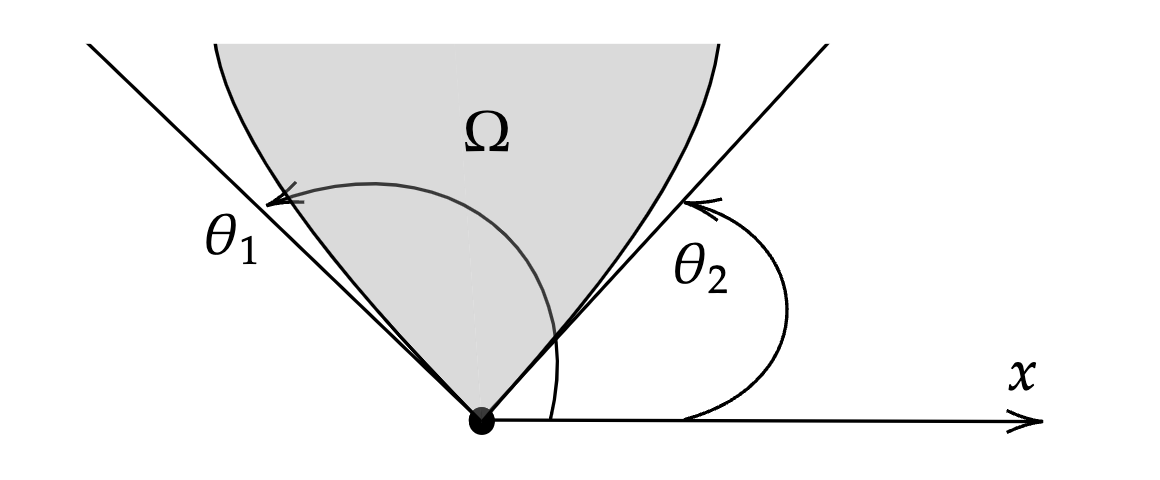
\includegraphics[width=0.6\textwidth]{angle}
    \caption{Solid angle related to a corner point of a nonsmooth boundary.} 
    \label{fig:angle}
\end{figure}

Equation~\eqref{eq:bie} is an integral equation on the boundary $\Gamma$, that is a \emph{boundary integral equation} with which it is possible to derive the potential where its normal derivative is known, and viceversa.

Indeed, assuming smooth boundary, by explicitly writing the boundary conditions we obtain two separate equations
\begin{align}
\frac{1}{2}\ \overline{u}=-\int_\Gamma \left( G\ \frac{\partial u}{\partial n} - \overline{u}\ \frac{\partial G}{\partial n}\, \right) \, \mathrm{d}S, \label{eq:u-known} \\
\frac{1}{2}\ u=-\int_\Gamma \left( G\ \overline{u}_n - u\ \frac{\partial G}{\partial n}\, \right) \, \mathrm{d}S. \label{eq:un-known} 
\end{align}

\subsection{BIE for the Poisson Equation}
\label{sub:BIE_for_the_poisson_equation}%

We briefly mention that in the case of Poisson equation, the BIE is turned into
\begin{equation*}
\frac{1}{2}\ u = u_0+u_1 
\end{equation*}
where $u_0$ is the already found solution of the homogeneous equation (Laplace equation) and $u_1$ is a particular solution, i.e. any function that satisfies only the governing equation $\Delta u_1=f$ independently of boundary conditions. Hence, by defintion of the fundamental solution, we simply have
\begin{equation}
\label{eq:PassoAsso}
u_1=\int_\Omega G\,f\ \mathrm{d}\Omega.
\end{equation}











